\documentclass[sigchi, nonacm, balance=false, authorversion=true]{acmart}
\usepackage{enumitem}

\graphicspath{{./Graphics/}}
\begin{document}

\title{Improving technical debt management and communication by visualizing source code}
\subtitle{A concept driven design study to expore the concept of a visualization tool to improve technical debt management and communication}
\author{Axel Ekwall}
\email{axelekw@kth.se}
\affiliation{%
  \institution{KTH Royal Institute of Technology}
  \city{Stockholm}
  \country{Sweden}
}


%% max 300 words

\begin{abstract}
With our increasing reliance on digital technology in our lives, we more than ever before depend on software products and services and the development of such products and services is becoming more complex and sophisticated. 
In these large software projects, developers often has to make compromises or settle for less than optimal solutions in order to reach deadlines or deliver a product to market in time.
This can cause what is known in the industry as \textit{Technical debt}, the accumulation of cost created by these "shortcuts" taken during development.

The goal of this paper is to design a concept of a visualization tool to aggregate and present an overview of technical debt in a software development project.
Based on this goal, the study tries to answer the following question: \textit{Can a visualization tool help software development teams manage technical debt by improving awareness and communication about technical debt strategy and priorities?}.

A literature study on the topics of technical debt management and information visualization techniques was conducted in order to create a foundation for the work in this project.

By leveraging \textit{concept driven design research} \cite{stolterman_concept-driven_2010}, a survey was conducted and based on the results, an interactive prototype was developed to evaluate in order to answer the research question.
The prototype was evaluated through critique sessions with semi-structured interviews with expert users working in software development projects.
The main findings are that a visualization tool, like the concept proposed in this study, could be used to help developers and other stakeholders in software projects raise awareness about technical debt strategies and priorities.
However, more research are required in order to refine the tool and visualizations included in the prototype.

\end{abstract}

\keywords{information visualization, technical debt management, concept driven design research}

%%
%% This command processes the author and affiliation and title
%% information and builds the first part of the formatted document.
\maketitle


%% ~1 page

\section{Introduction}
In recent years society has undergone a digital transformation and our everyday life depends on digital technology more than ever before. 
This development relies on an ever-growing collection of software systems and services that span our society and connect our lives. 
With the increasing size and scope of these software projects, and the growing numbers of software developers working in the same project simultaneously, development planning and collboration becomes harder. //SOURCE
A common method to handle these challanges is for software development teams to work according to an agile methodology \cite{hazzan_agile_2014} where requirements and solutions in a project are evolving over time in collaboration between developers, project managers and users. 
This process is conducted in an iterative cycle with continuous reflections and improvements on previous work.

In order to handle these iterative and fast paced change to the source code in a project, development teams are using version control systems to keep track of changes. 
This allowes developers to work on different versions of the software in parallel and \textit{commit} their changes to the project in batches when new features are completed or bugs are fixed.
All these small incremental changes are recorded and make up a rich source of information into the evolution of the code. 
However, this information is cumbersome to grasp and oversee and therefore often not used in an effective way, partly because it is not aggregated and presented as relevant metrics, but also because it is hidden from non-technical stakeholders who might not be able to retrieve the information from the VCS system. //SOURCE
This makes it hard for stakeholders to get an overview of how the project in general, and more specifically the source code, evolves over time.
In this context, where rapid continuous decision making and reflection is important, insights into the evolution of the source code and a shared understanding of the current state of the code can be valuable. \cite{ball_if_1997}

\subsection{Information visualization}




\subsection{Technical debt}
A term commonly used to describe this type of issue which might arise in large projects is technical debt, describing the increasing cost of development over time in a poorly maintained software project. 
The term, first described by Cunningham in 1992 \cite{cunningham_wycash_1992}, is a metaphor to financial debt in the sense that a development team might increase their technical debt by taking shortcuts in the development in order to save time in the short term.
However, this debt can be costly of not payed back in time by going back and refactoring parts of the code that might be sub-optimal.


\subsection{Research question}

The goal of this paper is to design a concept of a visualization tool to aggregate and present an overview of technical debt in a software development project.
In doing that, his thesis aims to investigate whether a information visualization tool can be used to empower software development teams to make better informed decisions about software architecture and source code maintenance on order to manage technical debt.
Based on this goal, this paper will try to answer the following question.

\smallskip
\textbf{
Can a visualization tool help software development teams manage technical debt by improving awareness and communication about technical debt strategy and priorities?
}
\smallskip

In order to answer the research question, a prototype of a visualization tool will be developed and evaluated based on the following sub-questions:
\begin{itemize}
\item Does the prototype present enough information for developers to make decisions about if and when to pay off technical debt?
\item Can the prototype help improve awareness about technical debt strategy and priorities within a software development team?
\end{itemize}

\subsection{Delimitations}
The main objective of this study is to evaluate a design concept, not developing a fully functioning visualization tool.
Only the features and interactions necessary to properly evaluate the concept and generate design guidelines will be implemented in the prototype.
\section{Related research}
To be able to design and develop the prototype of a visualization tool to help manage technical debt, previous work in relevant fields of research was reviewed.
This section presents and reviews the research from two main areas, technical debt management and information visualization, upon which this study builds.

\subsection{Technical Debt}
First described by Cunningham in 1992 \cite{cunningham_wycash_1992}, technical debt is a metaphor to financial debt and describes the common situation with increased development costs over time in software projects caused by poor software engineering practices \cite{tom_exploration_2013}.

Over time, the concept of technical debt gained in popularity and with that the scope of the metaphor was expanded to include any imperfection in the software lifecycle.
With this broader definition of technical debt, the need for strategies to monitor and manage the debt in a project are created.
Seaman and Guo, in the paper \textit{MEASURING AND MONITORING TECHNICAL DEBT}, proposes a "technical debt list" with "debt items" in order to monitor and keep track of instances of debt present in the project \cite{seaman_measuring_2011}.

The notion of a "debt item" will be used in this study to represent the debt in a project and present an overview to developers and other users of the proposed tool.
The "debt item" described by Seaman and Guo includes a description of where in the system the debt is present and why the task needs to be payed off \cite{seaman_measuring_2011}.
In this study the concept is expanded to also include the type, or dimension of debt the item represents.

The idea of \textit{debt dimensions} was introduced by Tom et. al. in their exploration of the technical debt definition \cite{tom_exploration_2013}.
Through a multivocal literature review of the current technical debt literature as well as interviews with participants from industry, Tom et. al. proposed five distinct dimensions of technical debt; \textit{Code debt}, \textit{Design and architectural debt}, \textit{Environmental debt}, \textit{Knowledge distribution and documentation debt} and \textit{testing debt} \cite{tom_exploration_2013}.
Further, Tom et. al. also explores the factors that contributes to technical debt in projects and among them they identified the following main factors; \textit{Pragmatism}, \textit{Prioritization}, \textit{Process}, \textit{Attitudes} and \textit{Ignorance} \cite{tom_exploration_2013}.

Of special interest to this study are \textit{Prioritization}, \textit{Process} and \textit{Attitudes} since these are factors that are addressable through a visualization tool.
Tom et. al. writes, "The visibility of all forms of technical debt decreases when poor communication and collaboration processes are in place, making it easier for debt to accumulate without being noticed." \cite{tom_exploration_2013} suggesting that visibility and communication are key to establishing a successful technical debt management process.

Worth noting when when dealing with technical debt is that, even though concept in many ways are associated with negative effects, in some cases, taking on technical debt can be a strategic short term decision in order to reach a critical deadline in time.
However, if not properly managed the debt can be costly by decreasing development velocity and increasing maintenance costs \cite{seaman_using_2012}.

\subsection{Information Visualization}
The core of information visualizations are the mapping of data and intent to visual representations.
Although there are many different techniques used in the field, this central process of visualizations can be described by the \textit{Reference model for visualization} by Card et al. presented in figure \ref{fig:vizprocess} \cite{card_readings_1999}.
This common reference model is helpful in order to analyze and compare the different techniques as seen in the taxonomy proposed by Chi based on model by Card et al. \cite{chi_taxonomy_2000}.

\begin{figure}[t]
  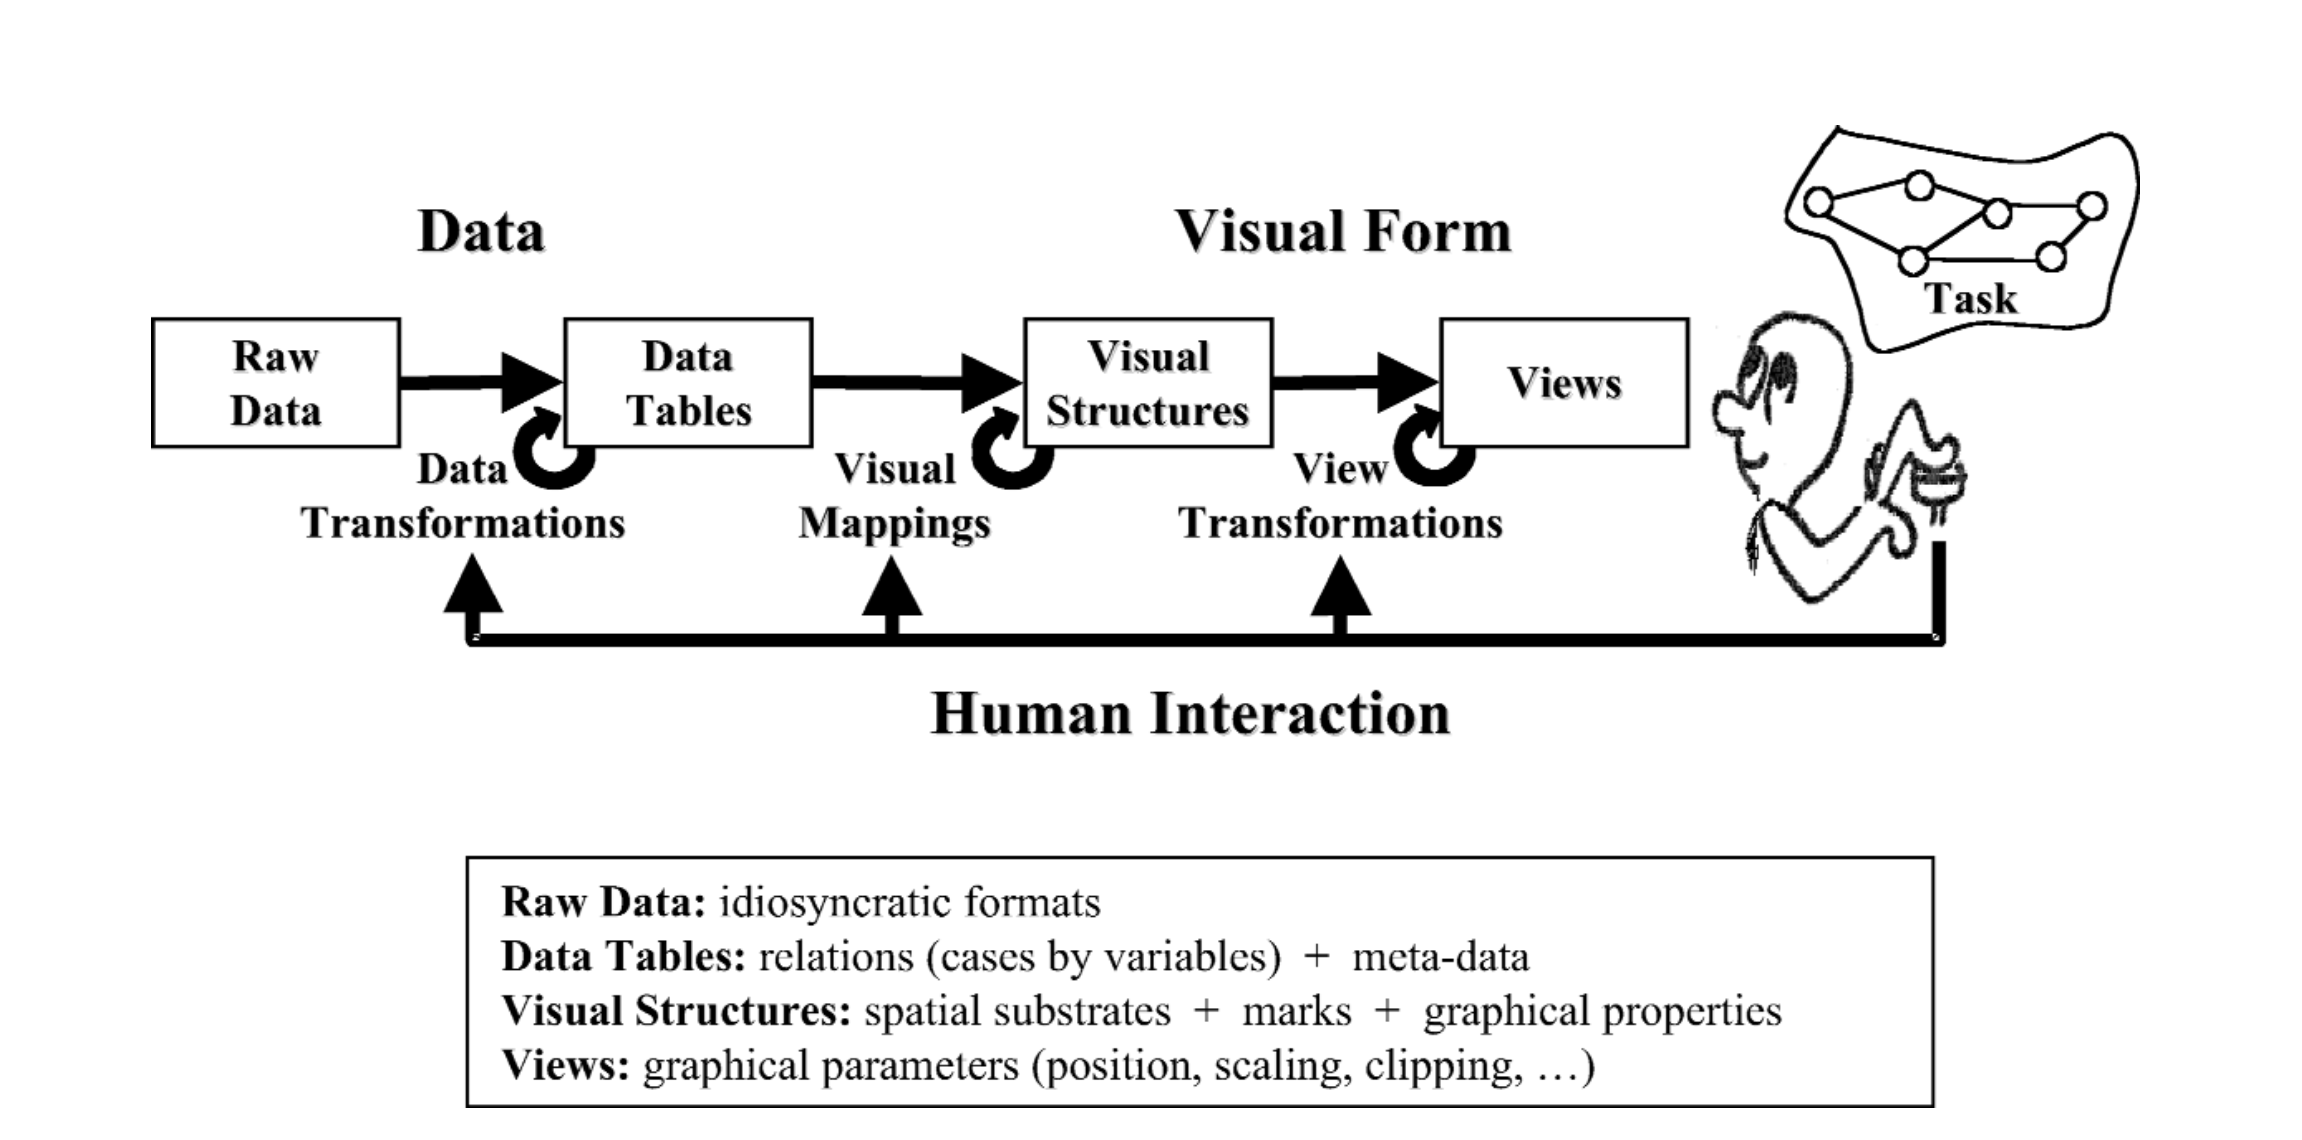
\includegraphics[width=\columnwidth]{VisualizationProcess}
  \Description{Chart over the Reference model for visualization by Card et al. 1999}
  \caption[Reference model for visualization]{Reference model for visualization by Card et al. 1999 \cite{card_readings_1999}}.
  \label{fig:vizprocess}
  \centering
\end{figure}

The raw data can take many forms which can be classified intro three main categories based on its properties, \textit{nominal data} is simple data with some sort of label but no quantitative value, \textit{ordinal data} can be ranked according to some attribute and \textit{quantitative data} which support arithmetic operations \cite{card_structure_1997}.

In this study, the source code of a software project is visualized.
The source code is a collection of files and folders that translates into a hierarchical data structure with nodes where each node can contain, or link to, a set of child nodes generating a tree-structure.
Hierarchies are closely related to network data structures, with the main difference being that hierarchies does not contain any loops within the connections \cite{spence_information_2014}.
Techniques to visualize hierarchies has been a heavily researched topic going far back, and there are multiple approaches and techniques to consider which can be divided into two separate groups, according to a survey of the design space by Schultz et. al. \cite{schulz_design_2011}.
Explicit tree visualizations are visual representations where the relations between nodes are shown with explicit lines or arcs, whereas implicit tree visualizations uses properties such as adjacency and encapsulation to represent the relationship between parent and child nodes in more space efficient way \cite{schulz_design_2011}.

Further, within the implicit tree visualization category there are two main visualization techniques to consider, \textit{Treemaps} and \textit{Icicle plots}, which both allow for many different layouts in both 2D and 3D.
Originating from Venn diagrams, \textit{Treemaps} are the most commonly used technique and are constructed by nesting the child nodes inside the parent node using \textit{inclusion} to represent the relationship between nodes.
\textit{Icicle plots} improves of the depth aspect by leveraging adjacency to represent relationship between nodes \cite{schulz_design_2011}.

In a more recent study by Woodburn et al. in 2019, comparing \textit{icicle plots} with \textit{treemaps}, it was concluded that \textit{icicle plots} are preferable by users as they are more intuitive and uses the screen space more efficiently \cite{woodburn_interactive_2019}.
\textit{Treemaps} was found to result in slower performance and accuracy regarding hierarchy navigation and understanding \cite{woodburn_interactive_2019}.

% \begin{figure}[b]
  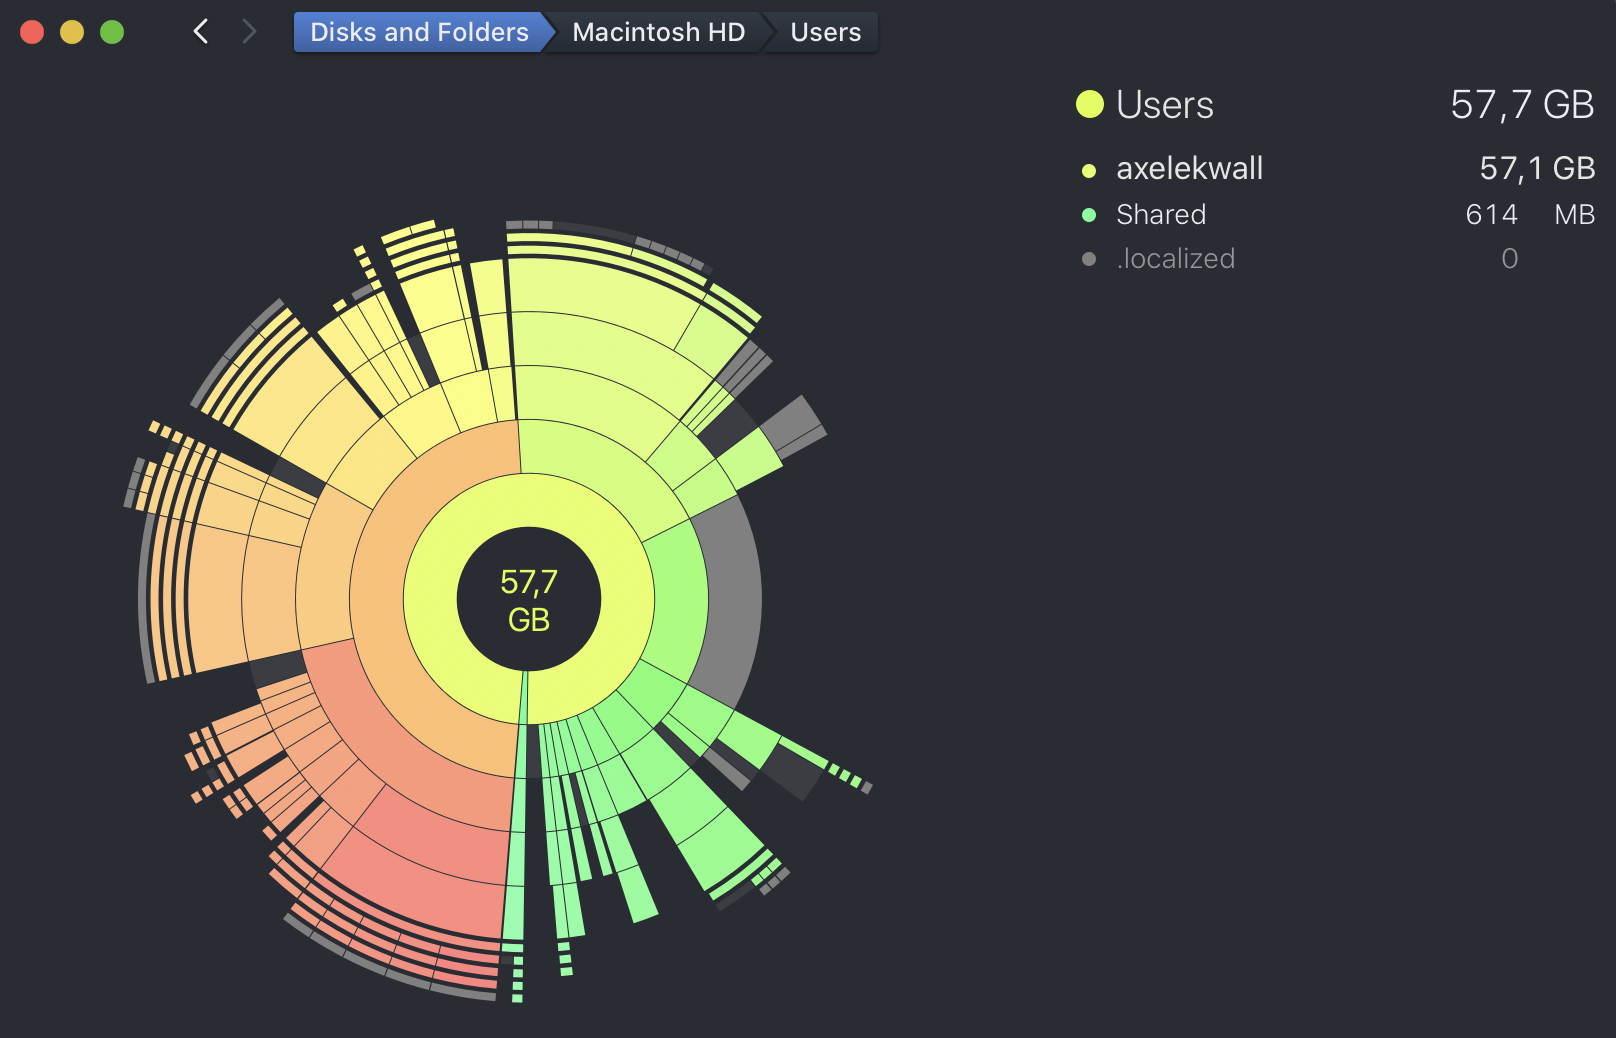
\includegraphics[width=\columnwidth]{example2}
  \Description{Visualization from the application DaisyDisk}
  \caption[Visualization example two]{Tree visualization from the application DaisyDisk representing the computers file system.}
  \label{fig:example2}
  \centering
\end{figure}
\begin{figure}[ht]
  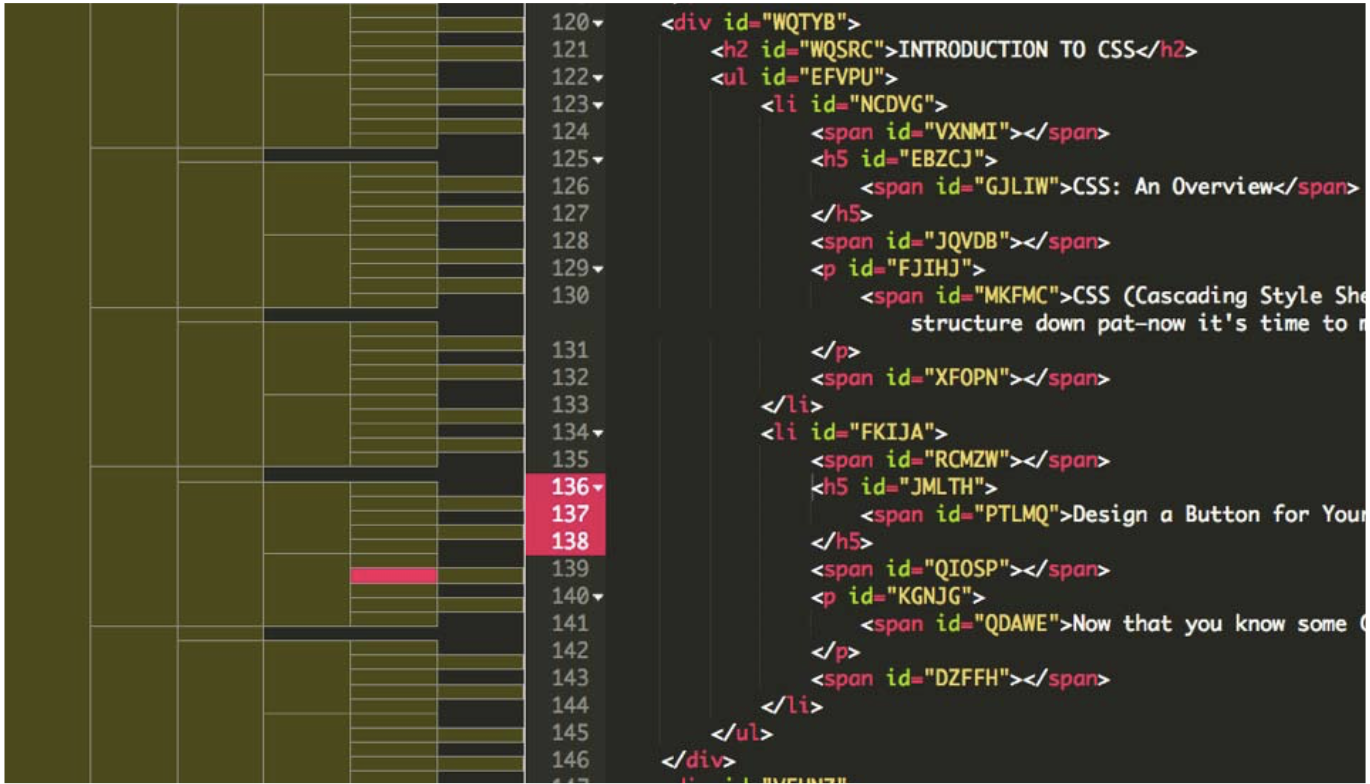
\includegraphics[width=\columnwidth]{example1}
  \Description{Visualization prototype from acher et al.}
  \caption[Visualization example]{Visualization prototype from Bacher et al. \cite{bacher_using_2016}.}
  \label{fig:example1}
  \centering
\end{figure}

There are multiple examples of tree visualizations to draw inspiration from.
Bacher et al. used both an \textit{isicle plot} and an \textit{circular treemap} to visualize source code in order to support comprehension, see figure \ref{fig:example1} \cite{bacher_using_2016}.
Further, based on the survey of the design space by Schulz et al. \cite{schulz_design_2011}, Schulz have gathered a collection of tree visualization examples categorized by dimensions of the design space available online at treevis.net \cite{schulz_treevisnet_2011}.
Lastly, there are examples with visualizations of multiple trees in the work by Graham and Kennedy \cite{graham_survey_2010}.


%% half page

\section{Method}
In this section the overall methodology used in this paper is presented. Each step is described in more detail in the next section "Study and results" together with the results.

TODO: Elaborate on the choice of method

In order to investigate the research question, a methodology informed by Stoltermans Concept-Driven Design Research (CDDR) \cite{stolterman_concept-driven_2010} was used with four methodological activities listed below.

\smallskip
\begin{enumerate}
  \item \textbf{Concept generation}, related literature study and survey gathering requirements.
  \item \textbf{Concept exploration}  and \textbf{design of artifact}, an interactive prototype manifesting the concept.
  \item \textbf{External critique session}, user study with prepared tasks and interview of target users.
  \item \textbf{Concept contextualization}, a discussion of the concept and results in this study positioning it against related research.
\end{enumerate}
\smallskip

As described by Stolterman in order for a concept to be valuable it should be based on previous theoretical work \cite{stolterman_concept-driven_2010}.
In this study, the \textbf{concept generation} is based on the theoretical work on \textit{technical debt} and \textit{information visualization} presented in the previous related work section as well as requirements gathered through a survey with respondents among potential users.
The survey was used in order to gather insight into the problems users face as well as their current processes and tools to manage and communicate about technical debt. 
The survey was conducted online and included an introduction of the topic, a section collecting background information about the respondents and two sections with questions.
In the first the respondents were presented with a collection of statements about their technical debt in their current project and were asked to evaluate their attitude on a Likert scale \cite{wilson_questionnaires_2013}, and in the second part the respondents were asked a set of open ended questions.

The next phase in this study was the combination of two activities, \textbf{Concept exploration}  and \textbf{design of artifact}.
During this phase, the form and functions of the concept was explored and an interactive prototype was designed and developed.
The prototype was developed with the purpose of testing new ideas of how to present technical debt in a software development project rather than refining current solutions or evaluating details in a design.
As Stolterman writes, "Concept design research does not strive to refine or test established ideas; instead, it explores new territories and design spaces" \cite{stolterman_concept-driven_2010}.

When the defined concept and features were implemented in the prototype, an \textbf{external critique session} was conducted in order to evaluate the concept manifested by the developed prototype.
The sessions were conducted online, one-on-one, with a video conferencing service and all sessions were recorded with video and sound for later analysis.
Each session followed a strict agenda starting with an introduction to the research project, concept and prototype read by the researcher followed by a section where the participant was exploring and interacting with the prototype by completing a set of predefined tasks.
These steps were conducted mainly to allow for the participant to understand and asses the prototype to be able to criticize the concept and the tasks were not designed to evaluate the usability or interaction with the application.

When the participant had completed the tasks and were familiarized with the prototype, a semi-structured interview was conducted.
In the first part of the interview, the participants were presented with four statements in order to spark a discussion about the prototype.
After each statement they were asked to discus their position regarding the statement.
The second part of the interview, the participants were asked a set of open ended questions about the concept in general.
After the interview were conducted, the data collected were analyzed using the \textit{thematic analysis} described by Braun and Clarke \cite{braun_using_2006}, and a collection of themes and sub-themes were discovered.

The last phase, \textbf{concept contextualization}, includes a discussion about concept evaluated in this paper and the knowledge gained, and tries to position it withing the landscape of previous research. This discussion is conducted in the fifth section of this report, and builds upon the findings from the study and results presented in the next section.

%% 4-5 pages

\section{Study and Result}

In this section the study will be described step by step in separate subsections in chronological order.
For each step, the method and results will be presented together.

%% The result will be divided into subsections for the result from the survey conducted to establish requirements and the results from the thematic analysis of the interviews conducted to evaluate a prototype of a proposed technical debt management tool.

\subsection{Survey}

The survey was conducted among professionals with various roles in software development projects, with the most common role being "Developer" (90\%) followed by "Tech Lead or Project Manager" (60\%) and "DevOps" (20\%).
The number of respondents was 20 with mixed and somewhat evenly distributed level of experience between "less than 5 years" (40\%), "between 6 and 10 years" (25\%) and "more than 10 years" (35\%).
All but one (95\%) of the respondents were familiar with the term "Technical Debt" indicating that the respondent have a understanding of the concept and thus the required prior knowledge to be able to provide relevant answers in the survey.

In order to understand how technical debt affects the daily work of the respondents and their experience of communicating about and manage technical debt in their current situation, the survey presented nine statements asking the respondents to indicate whether they agree or disagree according to a Likert scale. %% TODO: Add ref
The results are presented in figure \ref{fig:statementresult}, where each statement is assigned a letter and the distribution of the answers for each statement represented with a bar in the figure.

\smallskip
\textbf{Statements:}
\begin{enumerate}[label=\alph*)]
  \item I find that technical debt is a problem in my current project.
  \item Technical debt is often necessary in order to deliver in time.
  \item The amount of technical debt in my current project is acceptable.
  \item I have a clear overview of the amount of technical debt in the project.
  \item I have a clear overview of where in the project technical debt is present.
  \item The technical debt in the project is actively managed.
  \item The project team has clear communication about technical debt.
  \item The project team has a clear strategy for how to manage technical debt.
  \item Everyone in the project team are aware of the technical debt strategy.
\end{enumerate}
\smallskip

\begin{figure}[t]
  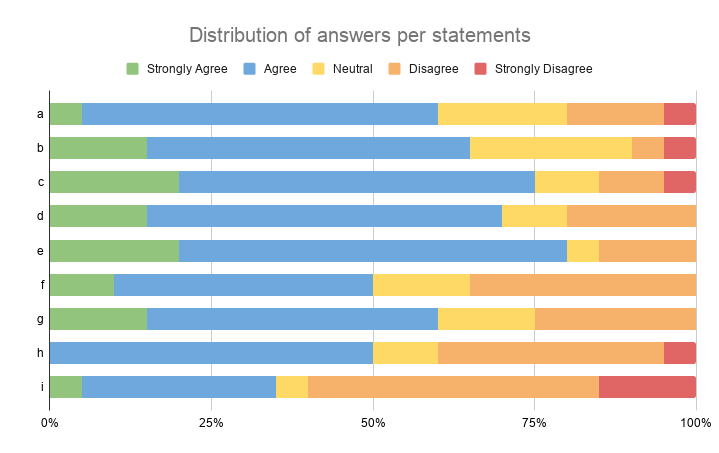
\includegraphics[width=\columnwidth]{StatementAnswers}
  \Description{Chart representing the distribution of answers per statement.}
  \caption[StatementResults]{Chart representing the distribution of answers per statement.}
  \label{fig:statementresult}
  \centering
\end{figure}

The results show that although more than half of the respondent (60\%) find technical debt to be a problem in their project, a majority (65\%) agree that technical debt is necessary in order to deliver in time.
Further, most respondents (75\%) consider their current level of debt acceptable.
This indicates that developers are facing the need to balance the problems caused by technical debt with the need to deliver in time and that this requires accepting a certain level of technical debt.

A greater part of the respondent indicate that they have a clear overview of both the amount of technical debt (70\%) and where the debt is located in the project (80\%).
However, only half of the respondents work in a project where technical debt is actively managed (50\%) or with a clear strategy for technical debt management (50\%), and a majority (60\%) does not experience that everyone in their team are aware of the technical debt strategy.
This points to a problem with an absence of awareness and communication about technical debt in many software development projects.

The second part of the survey included a collection of open ended questions about the respondents experience with technical debt in their daily work.
When asked how technical debt impacts their daily work the most common theme was that it leads to a slow down in the development process, results in longer time to deliver and limits the ability to add new features.
One respondent writes:
\begin{quote}
  "[It] takes longer time to deliver new features, onboard new team members, limits what solutions we can choose for problems." (respondent 17)
\end{quote}

Next, the respondents were asked to describe how they currently manage technical debt.
The most common answer was that they do it little by little as they stumbled upon it.
The "boy scout principle" was mentioned multiple times by different respondents.
One respondent explains:
\begin{quote}
  "Boy scout principle. Leave the code a little better than you found it." (respondent 11)
\end{quote}
Another aspect mentioned by multiple respondents is the difficulty managing a balance between paying off technical debt and adding new features as one respondent describes in the following statement: 
\begin{quote}
  "We write stories for it and add them to the backlog. Each sprint we include some such stories - but it's a bit of a tug of war with the business who wants more features instead." (respondent 16)
\end{quote}

When asked about what tools or processes the respondents currently are using to manage technical debt most of the respondents did not use any special tool but rather relied on their existing workflow for bug and feature tracking, code reviews and sprint meetings.

Lastly, the respondents were asked what features they would want in a tool designed to help manage technical debt.
Among the many different answers there were a few recurring suggestions for features or important aspects of such a tool.
Multiple respondents requested a way of understanding the balance between the cost of fixing instances of debt and the potential benefit gained by paying off the debt. An example is the following answer:
\begin{quote}
  "Wow, good question. Not sure, but I guess it'd important for me to somehow be able to see how 'expensive' a certain tech debt payoff project would be together with it's potential reward. This would make prioritization between different tech debt payoff projects better." (respondent 18)
\end{quote}
Another respondent describes a platform where you can document areas in the code where technical debt is present and keep track of the technical debt in the project:
\begin{quote}
  "A tool that could help us document part of the code we think as technical dept. A platform that we could have conversation about things and keep track of ideas how to solve things." (respondent 19)
\end{quote}
The idea of a tool to help a team schedule and prioritize technical debt also surface multiple times among the answers. One respondent writes:
\begin{quote}
  "Maybe a 'queue' of topics we have decided is tech debt and for how long they have not been addressed. Otherwise, a solution for the current standards and ways of working with notifications for 'now you have not reviewed this in X months'. Making a tool which proactively helps you schedule tech debt fixing which is open and transparent to both managers and developers." (respondent 15)
\end{quote} 

\subsection{Prototype}

TODO: More references to related work.

% In contrast, this study targets advanced users with domain knowledge and information about the context of the software project, allowing for a more advanced interactive visualization tool that presents complex information.

Based on the data collected and analyzed from the survey described in the previous section, a prototype of a tool was designed and developed.
One of the main takeaways from the survey is that a majority of respondents felt a lack of awareness among their team members.
Based on that finding, the goal of the tool is to raise awareness about technical debt among the team members of a development team, about the strategy, decisions and priorities regarding technical debt in a project.
Further, the tool also aims to be a common source of information about the technical debt in a project and to be a helpful tool in discussions and decision making.

The prototype was developed as a web application with modern web technologies, React and Redux, using the programming language Typescript.
In order to speed up the development process, a component library, \textit{Material-UI}, was used to create the overall structure of the interface.
It consists of a main view with a dashboard containing multiple widgets containing information about the technical debt in the project.
The widgets are interconnected and responsive to user interaction.
In order to facilitate the evaluation, the prototype was developed with static data and no integration with live projects.
However, the prototype is coded with real data in mind, and could be integrated with source code repositories with more development.

Based on the work by Seaman and Guo \cite{seaman_measuring_2011}, review in the related work section, technical debt is represented in the prototype as "debt items" which are instances of debt that can be assigned to a location in the source code.
Each debt item includes, in addition to the location in the project, also a title, description, deadline, type and priority editable by the user.
The debt \textit{types} used in this study are informed by the \textit{dimensions od technical debt} defined by Tom et. al. \cite{tom_exploration_2013}.

\begin{figure}[h]
  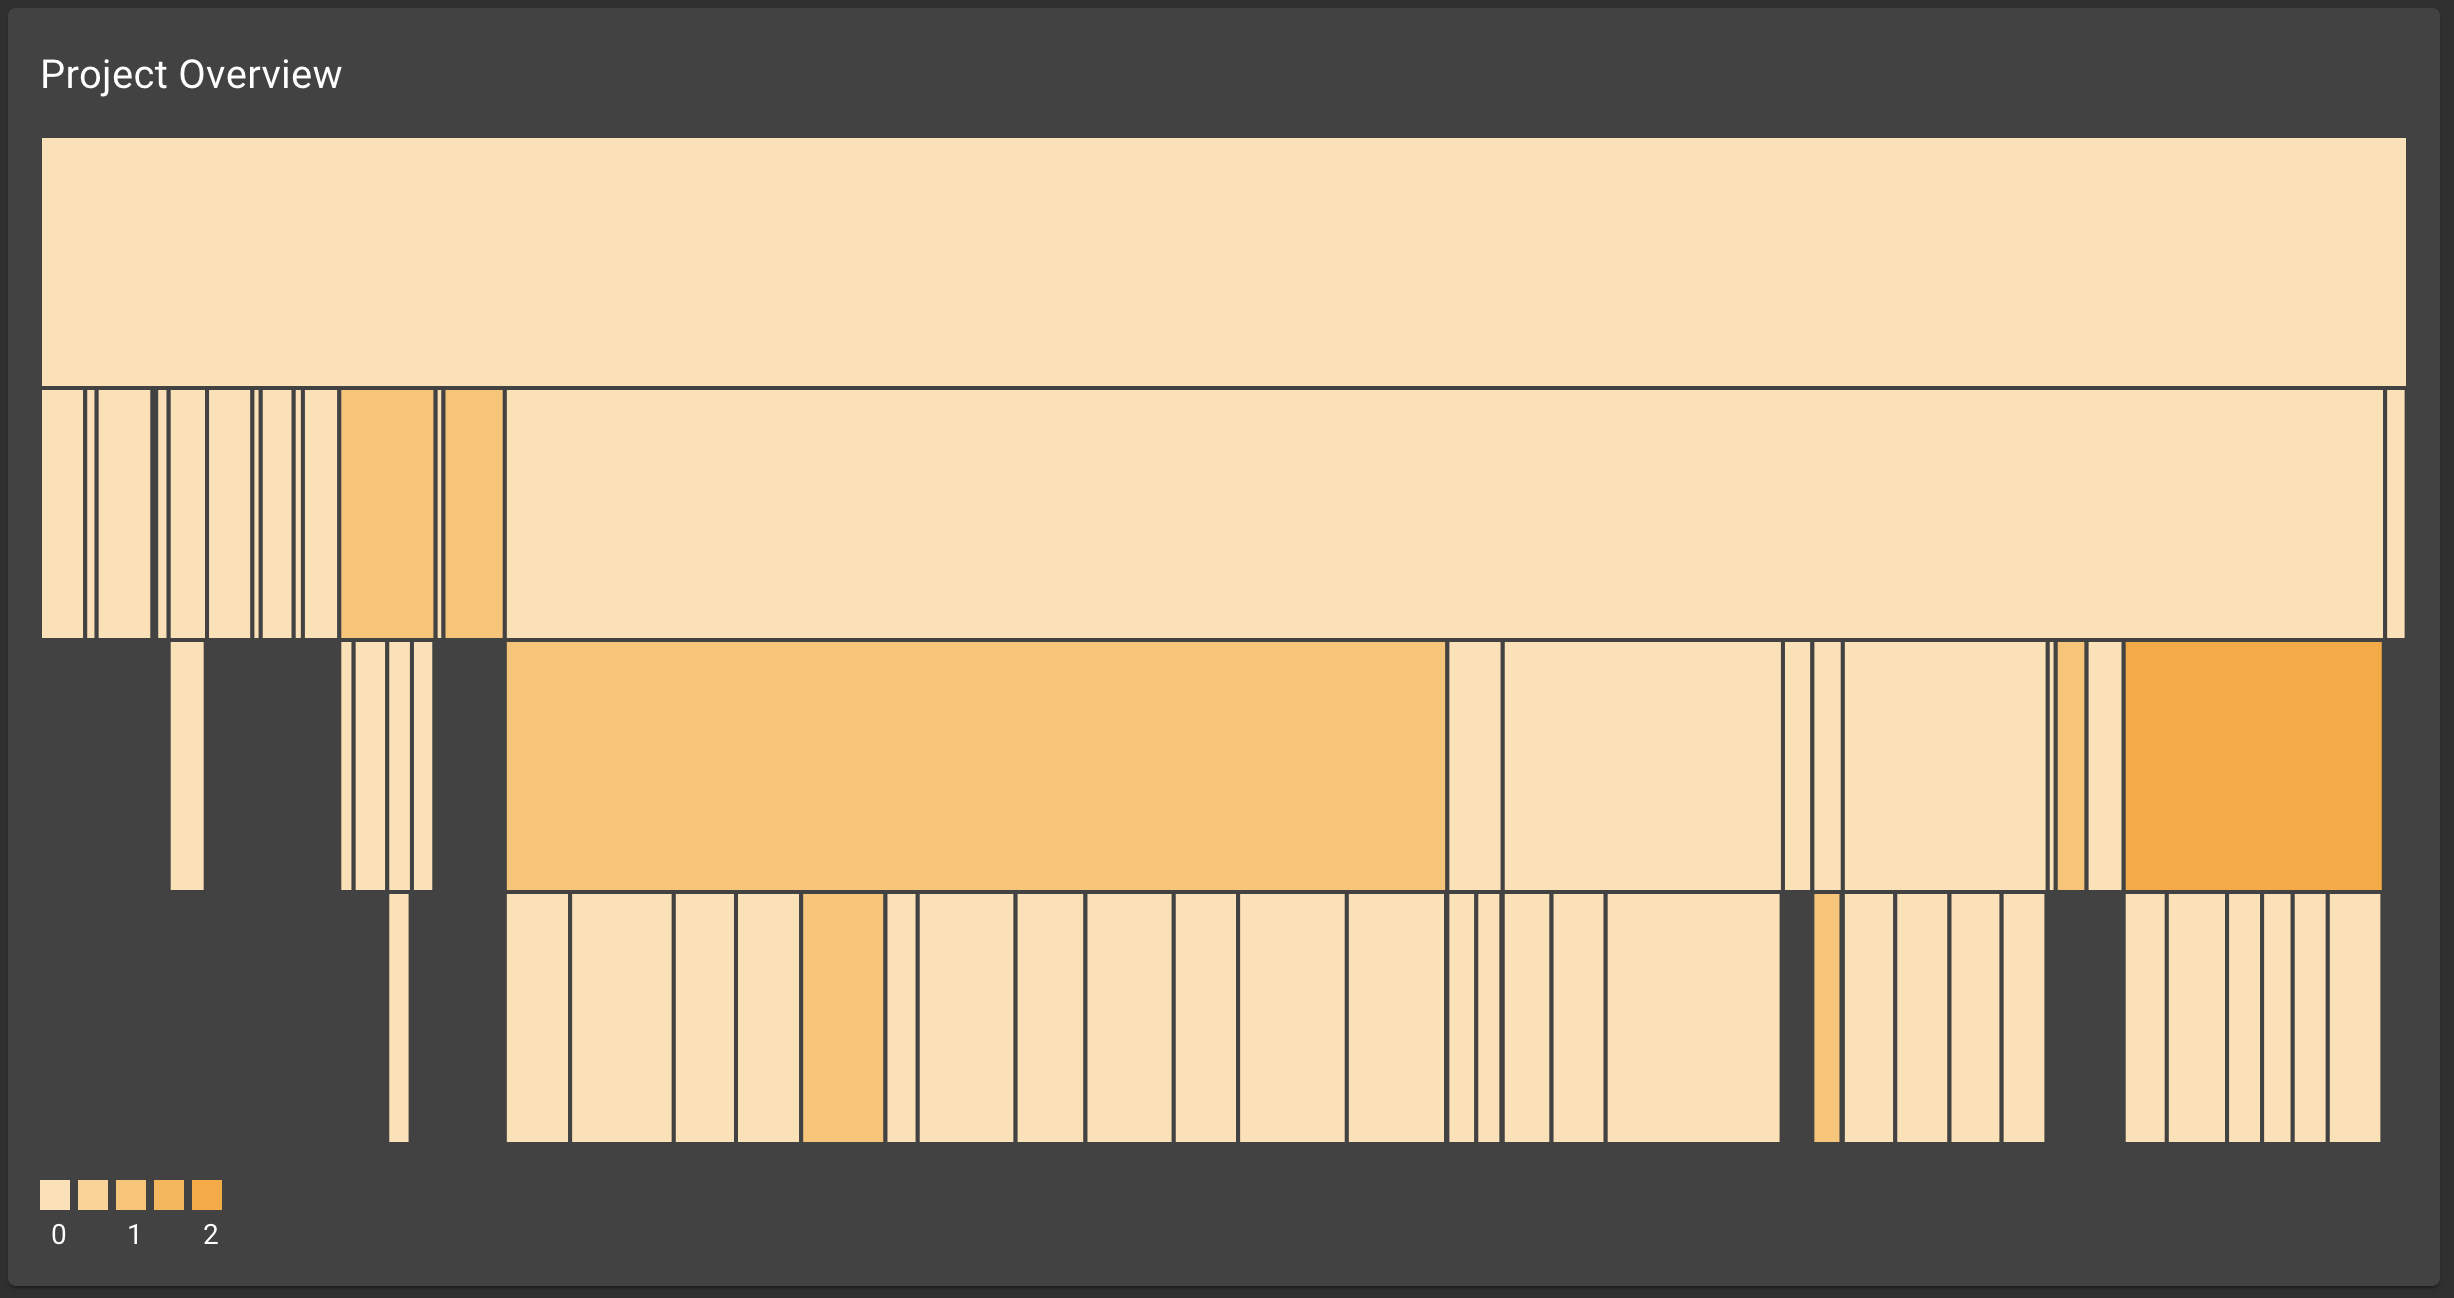
\includegraphics[width=\columnwidth]{overview}
  \Description{The overview visualization in the prototype.}
  \caption[Overview]{The overview visualization in the prototype.}
  \label{fig:overview}
  \centering
\end{figure}

The overview widget (figure \ref{fig:overview}) is a visualization of the source code represented as a partition layout.
Each file and folder in the tree structure is represented as a node, in this case a rectangle.
The layout is presented in a top down orientation implying that the top most node contains all nodes below it.
A node encodes three pieces of data, the location in the source code represented by the location in relation to other nodes, the size of the file or folder represented by the size of the node and the number of debt items associated with the node represented by the shade of the node.

\begin{figure}[ht]
  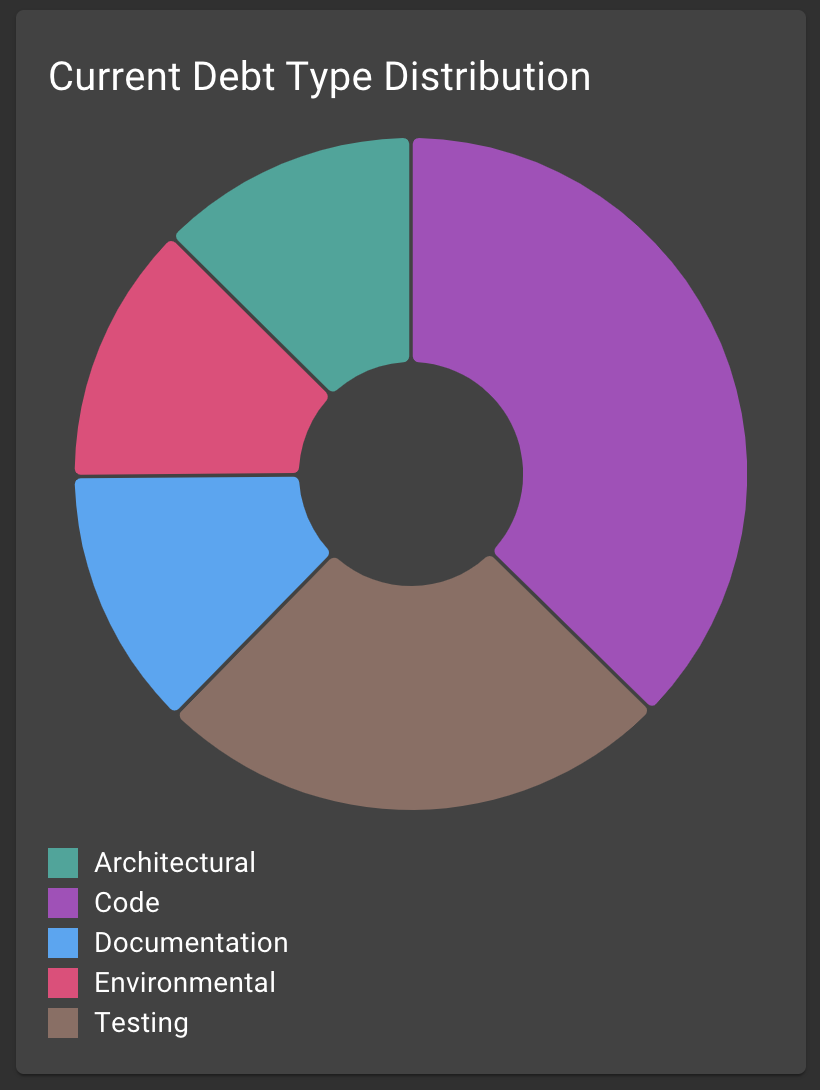
\includegraphics[width=\columnwidth]{debt-types}
  \Description{Prototype debt type visualization.}
  \caption[Debt types]{Prototype debt type visualization.}
  \label{fig:debt-type}
  \centering
\end{figure}

The debt type widget (figure \ref{fig:debt-type}) visualizes the distribution of debt types among the debt items in the project as a circle chart.
Each type corresponding to a distinct color which is recurring in other places in the prototype in order to help the user to find the type of a debt item at a glance.

\begin{figure}[h]
  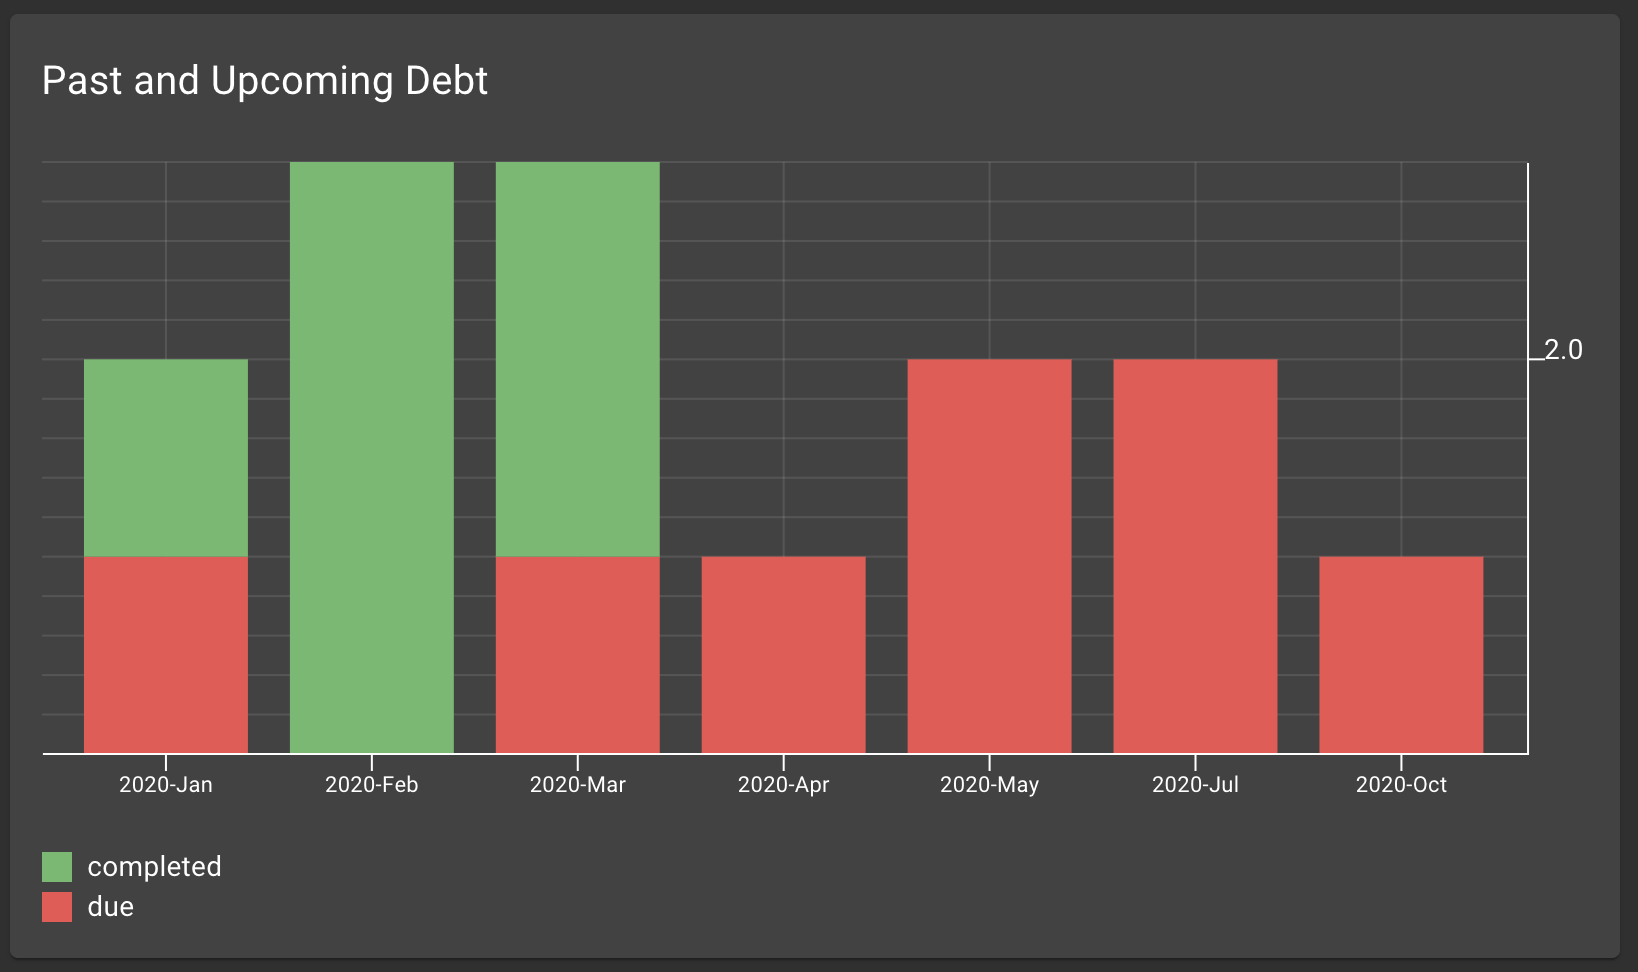
\includegraphics[width=\columnwidth]{history}
  \Description{The history visualization in the prototype.}
  \caption[Overview]{The history visualization in the prototype.}
  \label{fig:history}
  \centering
\end{figure}

To present the user with information about the evolution of debt in the project over a span of time, a timeline widget (figure \ref{fig:history}) is included in the prototype.
The timeline widget summarizes the number of debt items with deadlines for each month and visualizes this information as bar graph.
The bars include both completed (green) and non-completed (red) items colored by state.

\begin{figure}[h]
  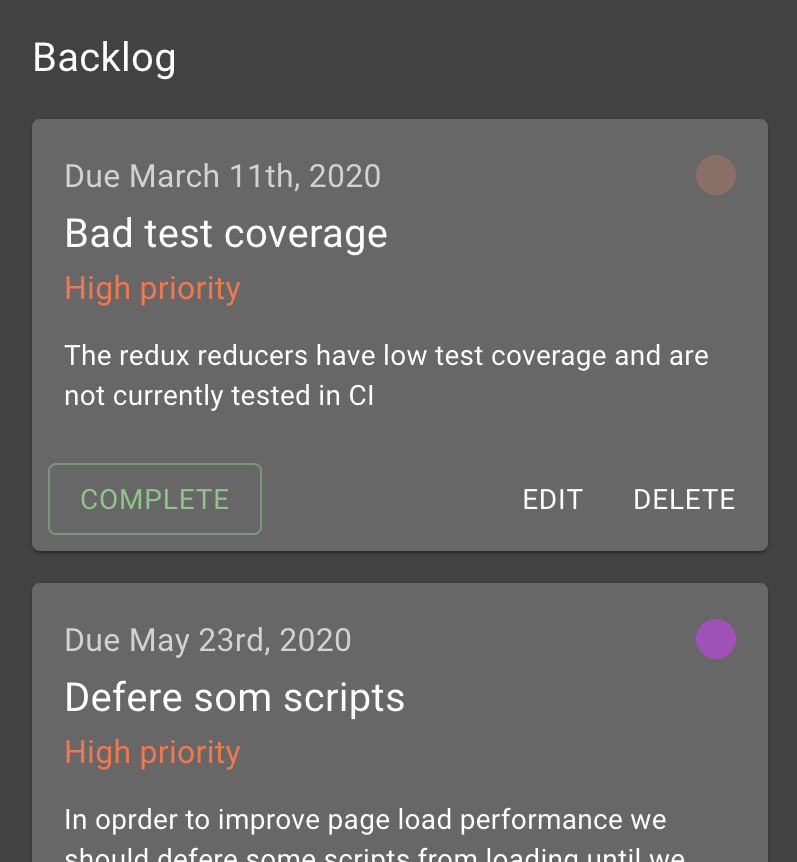
\includegraphics[width=\columnwidth]{backlog}
  \Description{The backlog column in the prototype.}
  \caption[Overview]{The backlog column in the prototype.}
  \label{fig:backlog}
  \centering
\end{figure}

The prototype also includes a column with cards (figure \ref{fig:backlog}) representing debt items, a "backlog" of items for the development team to work on. 
This is inspired by the approach proposed by Seaman and Guo where debt is presented as a "technical debt list" \cite{seaman_measuring_2011}.
The cards are sorted by priority and deadline with the highest priority debt items on top.
Each card presents all relevant information about a debt item and three action buttons: "complete", "edit" and "delete".
The user can also create a new debt item by clicking the button at the end of the list of cards.

The concept proposed in this study through this prototype aims to help development teams communicate about and manage technical debt by enabling everyone in the team to have an overview of the current technical debt status and priorities.
It allows the user to manage "debt items" representing an instance of debt somewhere in the project.
The user can create, edit and delete "debt items" which are presented as a backlog for the team to work on.
The user can also assign each item a deadline and priority. 
The goal is for this concept to be a common source of information about the teams strategy and priorities regarding technical debt, and also a help when making decision about technical debt in the project.
In other words, a unified interface for all kinds of debt in a project.

\subsection{Interviews}

The prototype was then evaluated through semi-structured interviews with users in which the users were able to interact with and explore the interactive prototype.

The participants were recruited from two companies working with software development.
Six participants from Mentimeter AB, a product company providing a SaaS solution for interactive presentations and three participants from Prototyp Stockholm AB, a digital agency developing digital products and services for clients.
The participants all has a background working in software development projects of varying size, and have roles such as \textit{developer} (9), \textit{tech lead} (7), \textit{designer} (1) and \textit{project manager} (1).
Experience among the participants are varying between \textit{up to 5 years} (4), \textit{6-10 years} (4) and \textit{more than 10 years} (1).

In the first part of each interview, after exploring the prototype, the participants were presented with the following four statements in order to spark a discussion about the prototype.
After each statement they were asked to discus their position regarding the statement.

\smallskip
\begin{enumerate}
  \item The prototype provides a good overview of technical debt in the project.
  \item The visualizations in the prototype provides useful information.
  \item The prototype provides clear information about the priority of debt items.
  \item This tool provides the information needed in order to make a decision about when to pay off debt.
\end{enumerate}
\smallskip

Most of the participants (TODO: x/10) generally agreed with the first statement.
However, multiple participants noted that some types of debt might not map well to the source code and thus not be well presented in the overview visualization.

The second statement received mixed opinions.
Almost all participants (TODO: x/10) agreed that visualizations in general do add value to the tool and were useful.
However, The specific visualizations in the prototype receive some criticism regarding both the interaction and the presented information. 
Multiple participants mentioned that the overview visualization (figure \ref{fig:overview}) was missing labels for the nodes in order to understand it better without having to interact and trigger the tooltips.
As with the first statement some participants noted that only visualizing the source files as an overview might be insufficient in order to show all kinds of technical debt, especially for environmental and architectural debt.
Regarding the other two visualizations, a majority of the participants wanted to be able to filter the backlog based on type and date in addition to the location by selecting a debt type in the circle chart (figure \ref{fig:debt-type}) or a month in the timeline bar chart (figure \ref{fig:history}).

Although the majority of the participants agree with the third statement about the priority of debt items, many ask for a sorting option for the backlog column (figure \ref{fig:backlog}) in order to make it clear that the column is sorted by priority.
In the current version of the prototype without a user selectable sorting option, many users took some time to realize that the backlog is sorted at all.
Further, one user points out that it would be valuable to be able to filter out all low and normal priority debt items from both the backlog and visualizations to be able to focus on high priority items in some situations.

The fourth and last statement generated more disagreement (TODO: x/10) compared to the previous statements and many participants were reluctant to agree with the statement.
The general response was that the decisions about when to pay off debt are complex and requires weighing many different business opportunities against each other and a tool like this simply cant capture all that.
With that said, most participants agreed that this tool would be a helpful addition in meetings and discussions about such decisions.
One participant explains:
\begin{quote}
  "Debt doesn't live in it's own little bubble where you can just pay off debt all day, you have to balance it against all the other items in a backlog." (participant 3)
\end{quote}
A feature many participants suggested that would help in that regard would be to add an estimated cost of paying off each debt item and the potential benefit of doing so.

After the initial statements, each participants was asked a couple of open ended questions in order to further explore their experience with the prototype and the broader concept of a tool like it.

\smallskip
\begin{itemize}
  \item Do you think a tool like this would improve communications about technical debt?
  \item Do you think a tool like this would make it easier to manage technical debt?
  \item What would be the most important feature of a tool like this?
  \item In what context would you use a tool like this?
  \item How would you improve this tool?
\end{itemize}
\smallskip

The recorded answers and discussions from the open ended questions were analyzed according the the guidelines of \textit{thematic analysis} by Braun and Clarke \cite{braun_using_2006}, and the following four themes emerged:
(1) \textit{A designated place for technical debt discussions and decisions}, (2) \textit{Flexible visual representation of software project with multiple levels of detail}, (3) \textit{Not another tool} and (4) \textit{Cost and benefit estimates}.
The themes captures the recurring opinions voiced by the participants and are summarized below with examples from the transcribes interviews.

(1) Multiple participants (TODO: x/10) mentioned the need for \textit{a designated place for technical debt discussions and decisions} and found that the prototype could fill that need.
Discussions around technical debt are many times held casually among developers and never recorded or structured and thus hard to follow up or base decisions on.
A platform or a tool that encourages these discussions and keep a record of the outcome of such discussions can be a valuable addition in a development teams workflow. 
TODO: Example quote.

(2) A large group of the participants (TODO: x/10) noted that in order to support the large variety in debt types and debt items possible in many project, the tool would need to adapt to multiple levels of detail.
Some debt items could require the ability to specify an exact line of code in a source file, while other debt items can span a whole repository of source code or multiple micro services.
This requires \textit{flexible visual representation of software project with multiple levels of detail}.

(3) A common opinion among the participants (TODO: x/10) was that a key factor to adoption of this tool in their team is how well it can integrate with their current workflow and tools.
"\textit{Not another tool}" to add to the already long list of services to keep up to date, unless it can bring enough value in relation to the cost of maintenance and learning.
For some of the participants, the solution would be to make it well integrated with their workflow, for example allow them to add new debt items directly from their code editor or use this as a dashboard for an existing issue tracker etc.
Other participants would rather have this tool be very simple to the point where it's so easy to use that it won't add much complexity to their process, and keep it separated from their other tools and services.

(4) When asked whether this tool could make it easier to manage technical debt, a recurring theme among the participants (TODO: x/10) was the need for a \textit{cost and benefit estimate} from each debt item.
Many participants noted that this is a complicated topic and one way of estimating might not translate to every project.
However, a way of assigning cost and benefit to items is necessary in order to priorities and make decision about paying off debt.

TODO: Add example quotes for all themes.


%% 1-2 pages

\section{Discussion}

This study aims to improve the managements and communication of technical debt in software development projects by introducing a visualization tool.
A concept of the visualization tool was developed using concept driven design research and an interactive prototype of the tool was designed and evaluated in order to answer the question: 
\textbf{Can a visualization tool help software development teams manage technical debt by improving awareness and communication about technical debt strategy and priorities?}

The findings from the study suggests that a visualization tool can improve the communication and management of technical debt, a majority of participants in the study thought a tool like the prototype would improve communication about technical debt and make management easier.
However, the study also finds that since technical debt always exists in the broader context of a project and a business with many competing priorities, technical debt management can be complex and can not be isolated from the rest of the development process.

In order to answer the main research question stated above, the prototype was evaluated based on two sub-questions.
The first question, \textit{Does the prototype present enough information for developers to make decisions about if and when to pay off technical debt?}, focused on the information provided by the prototype.
In general the participants did find the information provided in the prototype adequate, with one main exclusion being a metric of the cost and benefit of paying off each debt item.
Some participants did note that this information probably would be hard to define since there is no obvious unit in which to measure this.
A suggestion from one participant was to provide a basic scale from 1-5 to assign as a cost vs benefit metric to each debt item and let each development team decide for themselves what this scale implicates.
Another similar approach proposed by Seaman and Guo would be to enable a cost-benefit analysis borrowed from financial debt by including \textit{principal} and \textit{interest} estimates for each debt item \cite{seaman_using_2012}.
This would make it possible to compare and easily prioritize debt items as well as aid in planning, which multiple participants raised as a concern without proper estimates of time to pay off each item.

The second sub-question, \textit{Can the prototype help improve awareness about technical debt strategy and priorities withing a software development team?}, aims to help answer whether the prototype can help teams align on priorities and decisions and improve communication.
A theme that emerged from the interview was that without a designated forum and platform to record and structure discussions about technical debt, they tend to happen casually among developers in the day to day work.
It is of course not a bad thing to have these daily discussions among developers, but if the communication and decisions about technical debt never gets recorded or formally agreed upon by the team as a whole, it is hard to follow up and keep track of the accumulated debt.

According the the results from this study, a tool like the one proposed by this paper could be both a place to record and structure the teams strategy regarding technical debt, but also a tool to inform the team and make sure that everyone involved in a project are aware of the progress and priorities regarding debt.
Many participants said that this would be a very valuable tool to use in sprint planning meetings to update the team on the current status of debt in the project and agree on what to do next regarding technical debt.
It was also suggested that the tool could be used as a means of communication between developers and management with regards to budget, new features and long term project planning.

Further, regarding the visualizations presented in the prototype, even though a large majority of the participants did think the visualizations provided valuable information, there are some notable critique of the interface.
The debt type and timeline widgets were overall accepted without major objections.
However, the overview icicle plot did receive mixed opinions from the participants in the study, most notably that it would not fully capture all aspects and parts of a large software project, since it only represents the source code of a single repository.
This, in turn, does make it far less useful since it only provides an overview of a subsection of the possible technical debt in a project.
The combination of the breadth of technical debt problems that might arise and the complexity of large software architectures, a single visualization simply will not be enough.

One possible solution would be to remove the possibility to assign a debt item to a location in the project, and focus on providing visualization for the other properties of technical debt such as severity, cost and timeline.
With that said, the results in this study does show that the idea of providing an overview of the location does add value to the tool, and a better solution would be to explore the possibility to expand the interaction of the overview visualization and add more views and possibly more layers.
Since the different debt types operate on different "levels", where for example architectural debt might include several micro services and span multiple code bases and code debt often affects only a couple of lines of code in a specific file, a multi layer visualization could allow for the user to zoom into the visualization and be presented with details for the relevant type of debt on each level.
Furthermore, another point noted by the participants were the ability to view multiple source code repositories at the same time to manage debt for multiple projects together.
In order to provide this functionality, it would be of interest to investigate the possibility of implementing some of the techniques from the survey of multiple tree visualizations by Graham and Kennedy \cite{graham_survey_2010}.

\subsection{Method Critique}
The choice of method for this study came with some compromises due to the limited time frame and scope of the project.
Stolterman suggest to include an \textit{internal critique session} among the methodological activities in his description of \textit{concept driven design research} \cite{stolterman_concept-driven_2010}.
This activity was not included in this study due to time constraints, and thus it only included a single design iteration.
With an additional critique session before the external evaluation, the prototype would most probably been a better representation of the concept and in that also result in a more extensive evaluation of the idea.

Further, a larger number of participants from a broader recruitment population would enable conclusions to be generalized with more confidence.
Since the workflow and process can be different in different organizations, to just include participants from two organizations, as this study did, will not capture the whole picture of how the industry works with technical debt.
However, since this study was conducted during a global pandemic and most companies, including the two involved in this study, moved to a distributed remote working model, the recruitment of participants were significantly harder.
The pandemic also forced the method to include only remote evaluations, and no in person interviews or workshops as initially planned were possible.
\subsection{Future Work}

This study evaluated a concept of having a tool to manage technical debt by designing a prototype of such a tool and present it to users from a target group.
The design of the tool and the interaction supported by it needs to be further developed and evaluated in future studies. Here follows some suggestions of areas of further research.

The visualizations used in this study to represent a project was, according to many of the users in the evaluation, not able to fully capture all the complexity of a large software project.
Other visualization techniques do need to be evaluated in future studies to find a suitable representation, or collection of representations, that can fully capture a whole project and present a intuitive visual representation for users.
This would be necessary in order for a technical debt tool, like the one proposed in this study, to be able to present the user with a good overview of the magnitude and location of technical debt in a software project.

The filtering and sorting functionality and interaction could be further explored in future work.
There are many properties of debt items that can support filtering and sorting and the visualizations needs to support these data changes and visually reflect each state in an intuitive way for the user.

Further, the use of hierarchal data in overview widget could be further improved upon.
There are many interesting possibilities to explore more advanced aggregation of the data in the hierarchy and add multiple color encodings for the categorical aspects of the debt items.
Also, the current interface only provides information for the current point in time. However, the data includes temporal properties and a suggestion for further studies is to develop and evaluate whether the interface could support interaction in a temporal dimension, allowing the user to explore the technical debt status at different points in time.

Another possibility of improvement for a possible future study would be to allow the participants to explore their own projects rather than a sample project provided by the study.
This could possibly result in more meaningful detailed feedback based on real world workflows and projects.
A suggestion would be to include this in a future case study and explore whether the findings from this work could be built upon by letting a software development team use a tool like this for an extended period of time with real data.

%% max 300 words

\section{Conclusion}
TODO: Summarize the findings and the discussion. This should be pretty similar to the abstract.

%%
%% The acknowledgments section is defined using the "acks" environment
%% (and NOT an unnumbered section). This ensures the proper
%% identification of the section in the article metadata, and the
%% consistent spelling of the heading.

\begin{acks}
I want to thank Björn and Tino...
\end{acks}

%%
%% The next two lines define the bibliography style to be used, and
%% the bibliography file.
\bibliographystyle{ACM-Reference-Format}
\bibliography{thesisRefs}

%%
%% If your work has an appendix, this is the place to put it.
\appendix

\end{document}
\endinput
